\begin{abstract}
In this work an individual-based model of bacterial conjugation is presented and validated using the experimental data available. The model is further employed in analytical study of individual contributions of horizontal and vertical transfers and their effects on global conjugation rates. 
\end{abstract}

\section{Introduction}

In order to thoroughly understand how the plasmids are distributed and evolve in a bacterial population is necessary to separately identify the different aspects that affect the progression of cell to cell transmission and the invasion in the whole population. The final outcome of the process leading to the partial or total infection a bacterial colony can be seen as the sum of a set of contributions due to vertical and horizontal transfers as well as how much the metabolic burden contributes, as a negative feedback loop, to the pace of conjugative process. In the most elemental level, the rate at which the infection progresses depends on how many times every single cell can spread the plasmid, which hereafter we call intrinsic conjugation rate, it also depends on how fast the transmissions from donor cells to recipient cells and further retransmission from transconjugants cells can be accomplished.


\section{Model description}

The individual-based models suffer from the lack of a strong formal support and models are normally hard to be read, transmitted and reproduced elsewhere. In order to overcome such limitation we had used the protocol Overview, Design concepts and Detail (ODD) \cite{citeulike:2285571, citeulike:7890776} which has been proposed as a standard way to specify and describe IBMs.

\subsection{Purpose}

The objective of this model is twofold in the sense that firstly we wanted to develop a very simple model providing a good fit to experimental data obtained from wet-lab studies in order to serve as a predictive tool and then use the model to explore some aspects which are hard to observe directly in experimental studies of plasmid spread. The central aspect of model lies on the idea of a local or intrinsic conjugation rate that has been termed $\gamma_0$ which stands for the number of plasmid transfer events, or conjugations per encounters with plasmid free cells. The encounters are evaluated in the zone of direct cell contact which, in the computational domain, is a $3 \times 3$ Moore's neighborhood.  Once found the value of $gamma_0$ which provides the best fit to experimental data  the model can analyze the temporal evolution and the relative importance of horizontal and vertical transfer in the plasmid spread as well as the effect of secondary transfers performed by transconjugant cells and how these values are coupled to the transfer rates and the initial densities.


\subsection{State variables and scales}

The model comprises two entity types, namely the bacterial individuals or agents and environment. The environment contains the rate limiting amount of nutrient particles required for the cell metabolism and growth. All agents evolve in a computational domain defined by a $1000\times1000\mu m$ squared lattice divided in $10^6$ cells of $1\times1\mu m$ representing a real surface of $1mm^2$. In this model the {\it agents} representing bacterial cells are defined individually by two state variables, namely the {\it plasmid infection state} and the $t_0$. The plasmid infection states are $\mathcal{Q} = {R,D,T}$  and the transition function for conjugative plasmids, $\delta$ is presented in \eqref{eq:transitionmap}. For the {\it oriT} construction only the first rule applies since transconjugant cells are sterile. The $t_0$ is the time of cell birth or the time of the last cellular division, it is employed in the estimation of agent doubling time used in the division decision rule.

\begin{equation}
\label{eq:transitionmap}
  \delta = \left\{ 
  \begin{array}{l l}
    (D,R) \rightarrow (D,T)	\\
    (T,R) \rightarrow (T,T)	\\
  \end{array} \right.
\end{equation} 

Finally the environment will hold the initial nutrient concentration for every lattice cell.  In the model initialization a fixed amount of substrate particles will be distributed over all lattice sites.


\subsection{Process overview and scheduling}
 
The dynamics of bacterial conjugation is modeled as the sequential execution of following set of cellular processes: the shoving of cells avoiding the overlap between two adjacent cells, the conjugation process and finally, the cellular division.  The state variable update is asynchronous. The order of execution of this process is shuffled to avoid any bias due to a purely sequential execution of model rule base, see ~\ref{alg:proc-sched}. Plasmid transfer is modeled based on the average number of conjugations per encounters or collisions between individuals, we called this the intrinsic conjugation rate ($\gamma_0$). Taking into account that $gamma_0$ is a parameter hard to obtain experimentally we used the available experimental data to estimate plausible values.  

\begin{figure*}
\centering
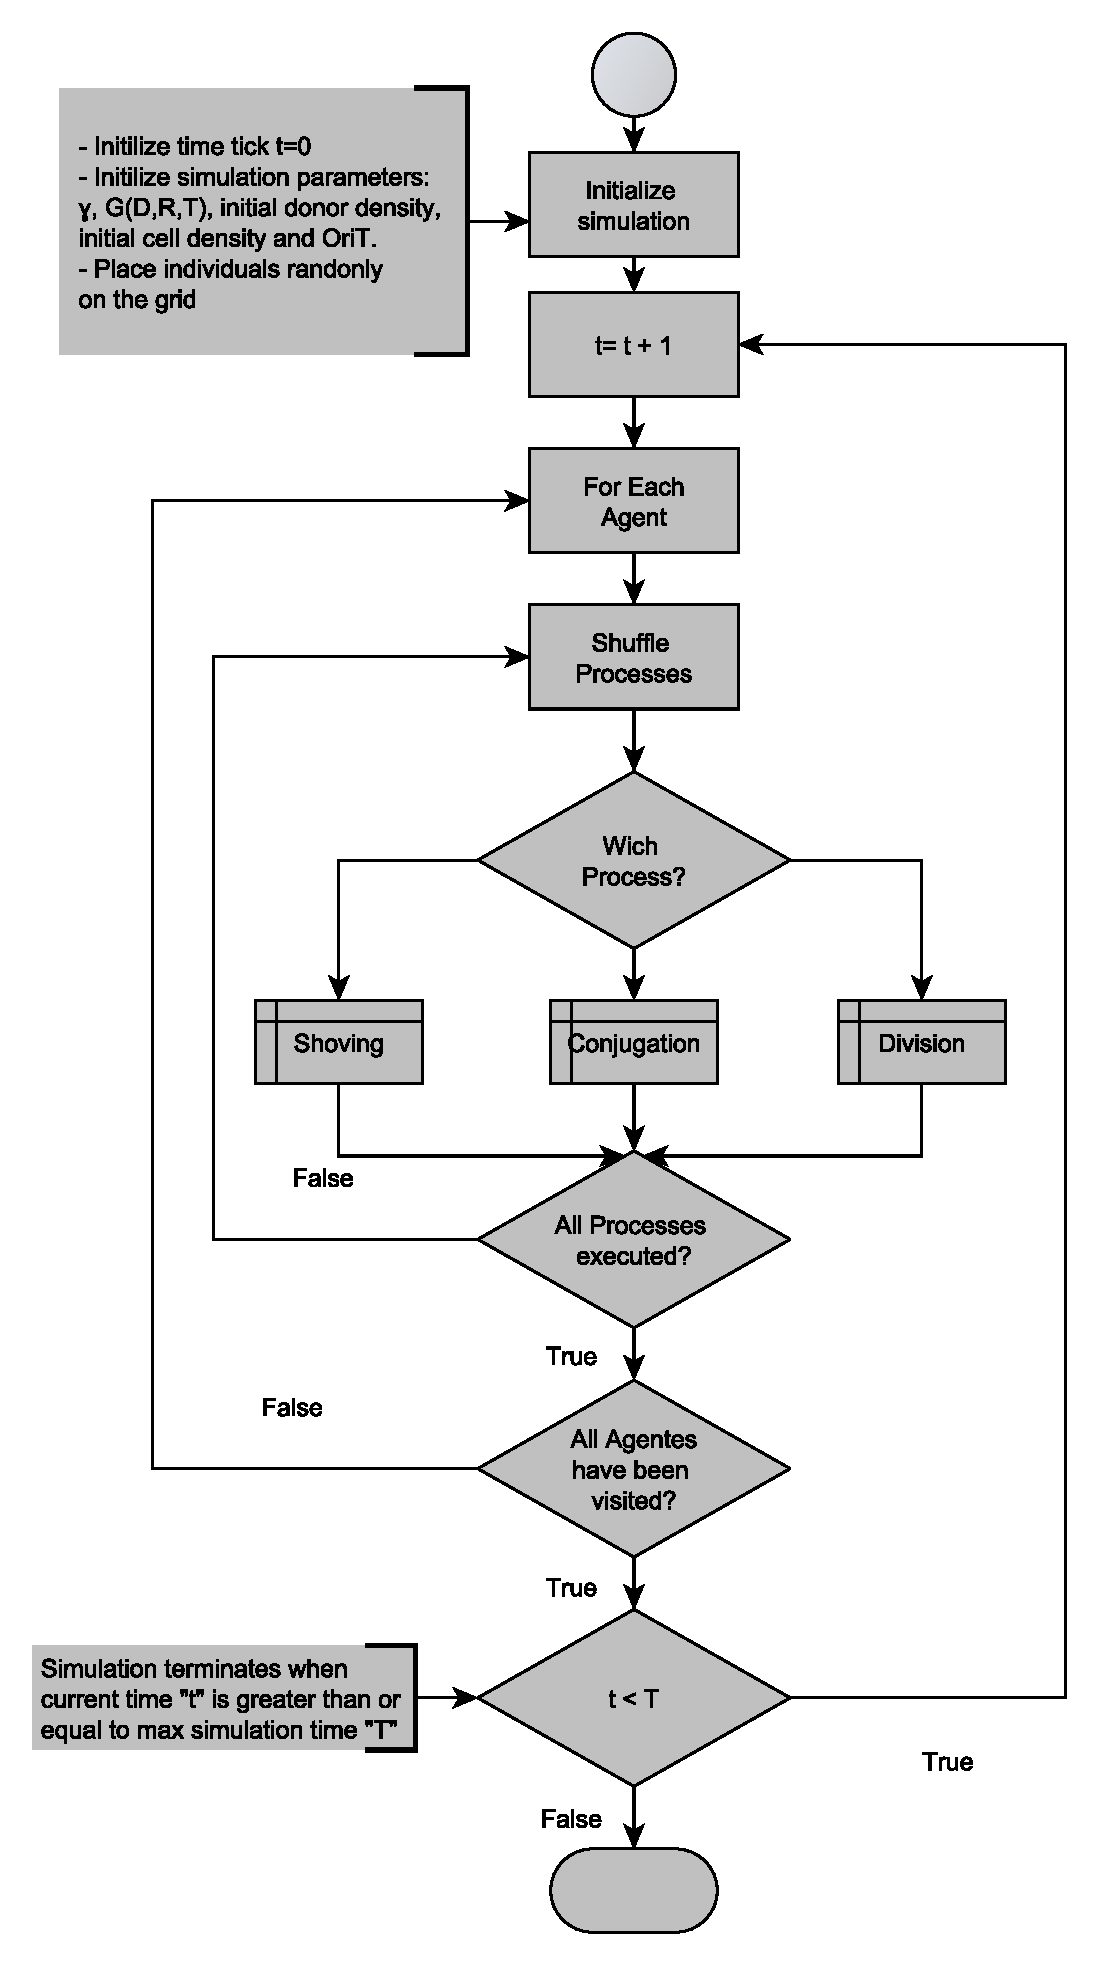
\includegraphics[scale=0.7]{m2-overview.pdf}
\caption[Process Scheduling]{\label{fig:proc-sched} Process Scheduling}
\end{figure*}


\subsection{Design concepts}
\
\\
{\bf Emergence} --- We want to find out what will be the global outcome which will arise as function of local rules defining the evolution of the bacterial cells and the interaction with other adjacent cells. With this objective, the model incorporates the most significant aspects of the structure and possible behavior of the structure as cellular processes that are interrelated. 
\\
{\bf Adaptation} --- All agents adapt their growth according to the local availability of nutrient and space.
\\
{\bf Fitness} --- It is considered implicitly to the extent that plasmid free individuals will present a better adaptation in terms of growth rate than plasmid bearing cells. Furthermore in one of the model executions we explicitly impose a fitness penalty every time that conjugation occurs in order to compare the resulting bacterial colony state.
\\
{\bf Prediction} --- The model is intended to provide prediction regarding the range of possible  values  for the number of plasmid transfer per cell cycle and the  cell cycle point when conjugative transfer are most likely to happen.
\\
{\bf Sensing} --- All process defined over the agents implicitly sense the local environment and the close neighborhood for their decisions.
\\
{\bf Interaction} --- Bacterial cells interact with their nearby individuals for nutrient access, cellular division, mate pair formation and plasmid transfer.
\\
{\bf Stochasticity} --- Stochasticity is introduced at individual level for all cellular process sampling a normal deviate and fitting the value to corresponding process.
\\
{\bf Collectives} --- No collectives are taken into account in this model.
\\
{\bf Observation} --- All state variables will be saved at intervals of fifty minutes of simulation.
\\
 
\subsection{Initialization}

The simulation model is initialized with an initial population of plasmid free $(R)$ and plasmid bearing $(D)$ cells according to input parameters. The agents are distributed randomly over a circular surface centered over the lattice central position. The radius of circle where agents are placed is calculated as function of $N_0$ in order to be consistent to the desired initial cell density. The simulation environment is also initialized with two nutrient particles.


\subsection{Input}

The model input uses the following parameterized list of variables:  The conjugation rate $\gamma0$ defined as the number of conjugations per encounters between donor and recipient cells. The average doubling time $\overline{g}(R,D,T)$ for plasmid free recipient cells $(R)$, for donor cells $(D)$ and for transconjugant cells $(T)$. The initial density of donor cells $(D)$ expressed as a percentage of total initial population $N_0$. The total amount of cells initially distributed in the simulation lattice $(N_0)$ expressed in cells/ml. Finally, the parameter {\it isOnlyOriT}, which allows the definition of mobilizable plasmids.


\subsection{Sub-models}

{\bf Nutrient Diffusion} --- The diffusion process uses the same approach described in \cite{citeulike:3567840} which is quite simple but effective capturing the essence and effects of diffusion process.  Roughly speaking, the technique allows nutrients to be consumed not just from local {\it lattice cell} but also from its neighborhood. Thus a size 3 {\it Moore's} neighborhood is used (a block of $7\times7$ lattice cells) for nutrient uptake but always giving priority to closer locations. Once the corresponding nutrient uptake is calculated, then try to retrieve such quantity from the local lattice site if possible. If there are no nutrients available at cell site select a random place at a neighborhood distance equal to 1, if nutrient concentration is greater than zero perform uptake from site if not remove from list and try again the same process at lattice distances of 2 and 3, if no nutrients are found return to some randomly selected lattice site at distance equal to one and repeat the process until find a site with a nutrient concentration greater than zero or when all sites were visited.  Such search is symmetric and makes nutrients closer to the bacterial cell position, much more prone to be consumed which in some extent emulates the real flow of nutrient particles towards clusters of bacterial cells due to resource depletion in such areas\cite{citeulike:3567840}. 

{\bf Nutrient Uptake} --- The uptake process always tries to consume one nutrient particle, assuming a simple functional dependence between the growth rate $\mu$ and the rate limiting substrate availability as can be seen in \eqref{eq:growth-rate}, that is to say when no nutrients are available the growth rate is zero and when substrate $S$ is greater than zero, the growth rate will be the maximum growth rate, as defined indirectly in the doubling time $(g)$ parameter. 

\begin{equation}
\label{eq:growth-rate}
  \mu(S) = \left\{ 
  \begin{array}{l l}
    S = 0, \mu(S) = 0		\\
    S > 0, \mu(S) = \mu_{max}	\\
  \end{array} \right.
\end{equation} 

\begin{figure}
\begin{algorithmic}[1]
\Function{Uptake}{}
\State $v \gets uptake(local)$
\If { v = 0 }
\State $v \gets uptake(diffusion)$ 
\EndIf
\State \Return v
\EndFunction
\end{algorithmic}
\caption[Uptake]{\label{alg:uptake} The Uptake rule}
\end{figure}

The complete nutrient uptake process is presented in ~\ref{alg:uptake} which basically shows that the local nutrient consumption will be tried first and in the case that local site contains no nutrient particles the aforementioned nutrient diffusion process is used.

{\bf Cell division} --- For each time step of simulation process a normally distributed random variable $Z_g$ with mean $\overline{g}(R,D,T)$ and standard deviation $\sigma_g$ will be generated as shown in \eqref{eq:division}

\begin{equation}
\label{eq:division}
\centering 
Z_g = \sigma_g Z + \overline{g},
\end{equation}

Where $Z_g$ is a random variable sampled from a standard normal distribution, the $\overline{g}(R,D,T)$  is the average doubling time for  plasmid free, donor and transconjugant cells respectively. The generated value $Z_g$ is then compared to the actual cell time defined as $\Delta_t = t - t_0$ being $t$ the current simulation time tick and $t_0$ the time of last cellular division.  

\begin{figure}
\begin{algorithmic}[1]
\Procedure{Division}{}
\State $\Delta_t \gets t - t0$
\If {$\Delta_t \ge Z_g$ }
\State $sites \gets getEmptyMooreNeighborhood(1)$
\If{ $size(sites) > 0$ }
\If{ $Uptake() > 0$ }
\State $t0 \gets t$
\State Divide()
\EndIf
\EndIf
\EndIf
\EndProcedure
\end{algorithmic}
\caption[Division]{\label{alg:division}The cellular division rule}
\end{figure}

Thus the effective division rule can be seen in Figure ~\ref{alg:division}.  First the current value of $\Delta_t$ is compared to $Z_g$ and, if it is greater than or equal to the estimated doubling time $g$ for the current agent the process continues and the availability of empty sites is checked.  Subsequently the agent will try to consume one particle of nutrient, first from current grid cell and, if there is no available nutrient in the local lattice site, the agent will try to consume the required nutrient particle using the diffusive process as described previously. Finally, if all conditions are met, a new daughter cell with the same conjugative state of the parent cell will be placed randomly at one of available empty sites.


{\bf Conjugative transfer} --- Every time a plasmid bearing cell, that is to say, donor (D) or transconjugant (T) bacteria individual\footnote{It is worth noting that T cells may or may not conjugate in our model and such behavior is controlled by {\it isOnlyOriT} parameter allowing to define a mobilizable plasmids}, meets an infectable recipient (R) the decision rule for conjugation compares the actual value of local $\gamma_0(local)$ to a normally distributed random variable $Z(\gamma_0)$ generated using the model parameter $\gamma_0$ and assuming a coefficient of variation equals to $0.1$ as can be seen in Equation \eqref{eq:zgamma0}.

\begin{equation}
\label{eq:zgamma0}
\centering 
Z(\gamma_0)= 0.1 \gamma_0 Z + \gamma_0
\end{equation}

Thereby the complete decision rule is shown in Figure ~\ref{alg:conjugation}. The code for performing conjugative events is pretty straightforward, we simply check for nutrient $(S)$ and infectable $R$ cells on the agent neighborhood and, if these conditions are satisfied, in the next step the current local $\gamma_0(local)$ is compared to the generated random variable. Thus the plasmid is transferred when the actual value of $\gamma_0(local)$ is less than $ Z(\gamma_0)$. When more than one recipient cell is available we randomly pick one of them.

\begin{figure}
\begin{algorithmic}[1]
\Procedure{Conjugation}{}
\If{ $S \ge 0$ {\bf and} $Neighbors(R) \ge 0$ }
	\If {$\gamma_0(local) < Z(\gamma_0)$ }
		\State Conjugate()
	\EndIf
\EndIf
\EndProcedure
\end{algorithmic}
\caption[Conjugation]{\label{alg:conjugation}The conjugation rule}
\end{figure}

The value of $\gamma_0(local)$ is estimated calculated for each agent using the expression shown in Figure \eqref{eq:zgamma0L} where $C$ and $E$ are respectively the number of conjugations performed by the agent and the number of encounters or "collisions" between the agent and $R$ cells on the neighborhood.

\begin{equation}
\label{eq:zgamma0L}
\centering 
\gamma_0(local)= \frac{C}{E}
\end{equation}




{\bf Shoving relaxation} --- In order to capture the effect of bacterial cells pushing each during the colony growth and expansion we had implemented a simple version of the shoving relaxation process. We are interested mainly on emulating the net effect of colony expansion in the modification of the local neighborhood structure besides of building a relatively realistic colony expansion pattern.  Our implementation assumes that bacterial cells are simple circular entities with a radius {\it r}. Although we are using a discrete grid with every agent occupying exclusively just one of the grid cells, the bacterial agents are allowed to have radius  with values greater than actual grid cell which actually is a square of $1\times1 \mu m$. 

Thus, the cell radius {\it r} is estimated using a simple linear relation between the current cell cycle point and the cellular elongation as shown in equation \eqref{eq:radius}.

\begin{equation}
\label{eq:radius}
\centering 
r= s_0 +  (s_g - s_0) \frac{\Delta_t}{Z_g}
\end{equation}

Where $s_0$ and $s_g$ are respectively the half of minimum cell size and the cell size at division, which are assumed to fall between $0.5$ and $3.0$ $\mu m$ for rod shaped cells.  

The shoving vector for every bacterial cell which overlaps with a neighbor is calculated in the same way as described in \cite{citeulike:464384}.  For every bacterial cell present in the computational domain we calculate a so called shoving vector using a Moore's neighborhood size 1, that is to say, accounting for the eight closest neighbors.  The shoving vector $\vec{s}$ is calculated as using the equation \eqref{eq:shoving}.

\begin{equation}
\label{eq:shoving}
\centering 
\vec{s}= \displaystyle\sum\limits_{i=0}^n \frac{kr + r_i - \Vert \overline{PN_i} \Vert}{2} \hat{u}_i.
\end{equation}

Where $\vec{s}$ is the shoving vector, $k$ is a constant used to set the maximum allowed distance or overlap between two adjacent cells, $r$ is the radius of current bacterial agent, $r_i$ is the radius of neighbor $i$, $\overline{PN_i}$ is the vector defined by the point centered at current cell and their neighbor $ i$ and finally $\hat{u}_i$ is the unit vector from the center of neighbor $i$ to the current cell. The bacterial cell position is then moved according to the vector $\vec {s}$. The rationale is to model the effect of passive movement of cells in the modification of the neighborhood structure which may facilitate plasmid donor cells to reach more individuals susceptible to be infected.

\section{Materials and methods}

For this work we have defined a set of simulated plasmids which parameters shown in Table ~\ref{tbl:plasmids}. These parameters are the bacterial cell average generation time $g(R,D,T)$ in the exponential phase, the initial cell density, the initial donor density and  a flag indicating whether plasmid is a repressed one ({\it repressed}), a flag permitting the definition of mobilizable plasmids which only has an oriT but lacks the TRA genes for conjugative transfer ({\it oriT}). Although not explicitly specified we are modeling low copy number plasmids. 

\begin{table}
\centering
\begin{tabular}{llllllll}
\toprule
Name 	& $\gamma_0$ & g(R) & g(D) & g(T) &  $N_0$(cells/ml) & $D_0$ & oriT \\
\midrule 
pR388 	& 0.5 & 43 & 42 & 46 & $5\times10^9$ & 5 & true \\ 
pR388 	& 0.5 & 43 & 42 & 46 & $5\times10^9$ & 50 & true \\ 
pSU2007 & 0.5 & 43 & 42 & 46 & $5\times10^9$ & 5 & false \\ 
pSU2007 & 0.5 & 43 & 42 & 46 & $5\times10^9$ & 50 & false \\ 
\bottomrule
\end{tabular}
\caption[Simulated plasmids]{\label{tbl:plasmids} Simulated plasmids parameters. The first parameter is the tentative value of intrinsic conjugation rate $\gamma_0$.  The following parameters are the doubling time $(g)$ for R, D and T cells. The $N_0$ is the initial population of the simulation experiment. The parameter $D_0$ is the initial donor density expressed in percentage of total initial population $N_0$. The oriT flag allow us to define mobilizable plamsmids where the conjugative machinery genes were knocked out. Thus when oriT flag is false, we are simulating a normal conjugative plasmid with and oriT and TRA+ genes, on the other hand, setting the flag to true allows the simulation of oriT construction, that is to say TRA-- non conjugative mobilizable plasmids. Perhaps parameter name is misleading mainly due to all simulated plasmids contains an oriT, but the real semantics is clear and should be read as {\it is the simulated plasmid an oriT construction where TRA genes have been deleted?}} 
\end{table}


To assess the distinct contributions of global conjugation rates we defined some new metrics and applied them in our simulated experimental setup in order to account for the relative importance of horizontal and vertical transfer and for the secondary transfers carried out by transconjugant cells. The first metric has been called {\it relative contribution of horizontal} transfer, henceforth $\mathcal{RC}_{\it h}$ and defined in Equation ~\ref{eqn:rch}.
\\
\begin{equation}
\mathcal{RC}_{\it h} = \frac{\sum \mathcal{D}_{\it c} + \sum \mathcal{T}_{\it c}}{\sum T} 
\label{eqn:rch}
\end{equation}
\\
We also define the metric {\it relative contribution of vertical} transfer ($\mathcal{RC}_{\it v}$ ) as the complement of horizontal contribution as shown in Equation ~\ref{eqn:rcv}.
\\
\begin{equation}
\mathcal{RC}_{\it v} = 1 - \mathcal{RC}_{\it h}
\label{eqn:rcv}
\end{equation}
Where the terms $\sum \mathcal{D}_{\it c}$, $\sum \mathcal{T}_{\it c}$ and $\sum T$ are respectively, the total number of conjugations performed by donor cells, the total number of conjugations accomplished by transconjugant cells and total number of transconjugant cells. This metric is the ratio of transconjugant cells which have been generated exclusively by vertical plasmid transmission to daughter cells.

Other metric defined in this work is the {\it relative contribution of transconjugant} plasmid transfer, hereafter $\mathcal{RC}_{\it t}$, which provides an indicator of the impact of transconjugant retransfer or secondary conjugation rounds performed by an initially plasmid free cell (R) that become a transconjugant (T) after have been infected. This metric is calculated as shown in Equation ~\ref{eqn:rct}.
\\
\begin{equation}
\mathcal{RC}_{\it t} = \frac{\sum \mathcal{T}_{\it c}}{\sum \mathcal{D}_{\it c} + \sum \mathcal{T}_{\it c}} 
\label{eqn:rct}
\end{equation}
With the objective of evaluating the intrinsic transfer rates, that is to say, the number of times that bacterial cells perform a successful plasmid transfer, the average number of conjugative events is also computed in our model. 

Another performance indicator defined in this work is the number of plasmid transfers per the total number of infected individuals, that is to say donor (D) or transconjugant (T) cells. Thus the indicator was termed $\gamma_i$ and is defined in Equation \eqref{eq:gammai}.

\begin{equation}
\label{eq:gammai}
\centering 
\gamma_i= \frac{C}{D + T}
\end{equation}

where $C$ is the total number of conjugative events and $D$ and $T$ the number of donor and transconjugant cells respectively.


\section{Results}

In the Table ~\ref{tbl:results} the averaged values of the seven replications of the simulation process are shown. Perhaps at a first sight the most interesting aspect that can be gathered from data are the discrepancies between the average values of $\gamma_0$ and the conjugation rate $T/(R+T)$. Intuitively could be expected the higher values of $\gamma_0$ intrinsic conjugation rates   would also lead to higher values of conjugation rates but that is not what is happening.  As can be observed the simulated plasmid pR388\footnote{The pR388 is a non-conjugative mobilizable plasmid which requires a helper conjugative plasmid in order to get transferred to other cells and the transconjugant cells generated in this way are sterile} at 5\% of initial donor density, have the highest $\gamma_0$ but also shows the lowest values of $T/(R+T)$  which in our simulations that has an average value of $0.10$. The next greatest value is shown by simulated plasmid pSU2007 at 5\% of initial donor density followed by pR388 having of $D_0$ equal to 50\% and finally, the lowest value of $\gamma_0$ is shown by pSU2007 at an initial donor density of 50\%. In order to understand these results let us see the meaning of the indicator that we are using. The $\gamma_0$ is the number of conjugations on an encounter basis, meaning that higher values indicates a very efficient transfer system coming to the case that a value of $\gamma_0 = 1$ is the perfect conjugative machinery where every time an infected cell  collides with a plasmid free cell a transconjugant is generated. 

\begin{table}
\centering
\begin{tabular}{lllllll}
\toprule
Name 	& $D_0$ & $\gamma_0$ & $\gamma_{ep}$ & $\gamma_i$ & $\frac{T}{R+T}$ &  $\overline{D}$ \\
\midrule 
pR388 	& 5		&  0.178 &  $5.65\times10^{-11}$ & 0.27 & 0.10 & 5.24 	\\ 
pR388 	& 50 	&  0.157 &  $8.11\times10^{-11}$ & 0.09 & 0.40 & 53.19 	\\ 
pSU2007	& 5 	&  0.161 &  $1.12\times10^{-10}$ & 0.35 & 0.31 & 35.05 	\\ 
pSU2007	& 50 	&  0.086 &  $4.96\times10^{-11}$ & 0.11 & 0.42 & 72.12 	\\ 
\bottomrule
\end{tabular}
\caption[Simulation results]{\label{tbl:results} Summarized results of simulation output. This table shows the average values of simulation model output.  The experimental plasmids pR388 (oriT) and pSU2007 were simulated at two levels (5\% and 50\%) of initial donor density ($D_0$). Thus the table shows the corresponding average values of conjugation per encounters ($\gamma_0$), the conjugation rate estimated by the end-point method ($\gamma_{ep}$), the  number of conjugative events per the total number of infected individuals ($\gamma_i$), the conjugation rate ($T/(R+T)$) and, finally de average value of the donor density. The $\overline{D}$ accounts for donor and transconjugant cells for conjugative plasmids or just for donor cells in the case of mobilizable plasmids (pR388).}
\end{table}


\section{Conclusions}